\documentclass[11pt,a4paper]{article}
\usepackage[utf8]{inputenc}
\usepackage{amsmath,amsfonts,amssymb}
\usepackage{graphicx}
\usepackage{geometry}
\geometry{margin=1in}
\usepackage{booktabs}
\usepackage{hyperref}
\usepackage{float}

\title{\textbf{EE3621: Digital Signal Processing} \\ \Large Lecture 22: Sampling Theorem, Aliasing \& A/D and D/A Conversion \\ \large (III B.Tech EEE)}
\author{Lecture Notes (40-Minute Plan)}
\date{}

\usepackage{xcolor}
\definecolor{darkbg}{HTML}{0d121f}
\definecolor{lighttext}{HTML}{e2e8f0}
\definecolor{primary}{HTML}{8b5cf6}
\definecolor{secondary}{HTML}{0dd5c5}

\pagecolor{darkbg}
\color{lighttext}

\hypersetup{
    colorlinks=true,
    linkcolor=secondary,
    urlcolor=secondary
}

\begin{document}

\maketitle

\section{Lecture Plan \& Objectives (40 Minutes Breakdown)}
\begin{itemize}
    \item \textbf{00:00 -- 05:00 (5 mins):} Introduction to Continuous-Time Sampling \& Mathematical modeling.
    \item \textbf{05:00 -- 12:00 (7 mins):} Nyquist-Shannon Sampling Theorem: Formal statement, proof, and conditions.
    \item \textbf{12:00 -- 17:00 (5 mins):} Aliasing phenomenon, folding frequency, and numerical example.
    \item \textbf{17:00 -- 22:00 (5 mins):} Practical ADC Pipeline: Anti-aliasing, Sample-and-Hold, Quantization.
    \item \textbf{22:00 -- 27:00 (5 mins):} Reconstruction (DAC): Zero-Order Hold (ZOH) droop and interpolation filters.
    \item \textbf{27:00 -- 31:00 (4 mins):} Oversampling ADC: SNR improvement and quantization noise spreading.
    \item \textbf{31:00 -- 35:00 (4 mins):} Sigma-Delta ADC: First-order and second-order noise shaping.
    \item \textbf{35:00 -- 38:00 (3 mins):} Sample Rate Conversion: Rational $L/M$ factor and polyphase implementation.
    \item \textbf{38:00 -- 40:00 (2 mins):} Checkpoints, Q\&A, and conclusion.
\end{itemize}

\noindent\rule{\textwidth}{0.5pt}

\section{Continuous-Time Sampling}

\subsection{Physical Intuition}
Sampling is the process of taking a continuous-time signal and measuring its value at discrete time intervals. Think of it like taking a stroboscopic video of a moving fan. If you take pictures fast enough, you capture the true motion. If too slow, the fan might appear to spin backward!

\subsection{Mathematical Model: Ideal Sampling}
We model the ideal sampling of a continuous-time signal $x(t)$ by multiplying it with an impulse train (or Dirac comb) $p(t)$.
\begin{enumerate}
    \item Let $T$ be the sampling period.
    \item The sampling frequency is $f_s = 1/T$.
    \item The impulse train is defined as:
    \begin{equation}
        p(t) = \sum_{n=-\infty}^{\infty} \delta(t - nT)
    \end{equation}
    \item The sampled signal $x_s(t)$ is the product:
    \begin{equation}
        x_s(t) = x(t) \cdot p(t) = \sum_{n=-\infty}^{\infty} x(nT) \delta(t - nT)
    \end{equation}
\end{enumerate}

\subsection{Frequency Domain Analysis (Derivation)}
To understand what sampling does to the frequency content, we take the Fourier transform of $x_s(t)$.
\begin{enumerate}
    \item The Fourier transform of a product in time is a convolution in frequency:
    \begin{equation}
        X_s(f) = X(f) * P(f)
    \end{equation}
    \item The Fourier transform of the impulse train $p(t)$ is another impulse train in the frequency domain:
    \begin{equation}
        P(f) = \frac{1}{T} \sum_{k=-\infty}^{\infty} \delta\left(f - \frac{k}{T}\right) = f_s \sum_{k=-\infty}^{\infty} \delta(f - kf_s)
    \end{equation}
    \item Substituting $P(f)$ into the convolution equation:
    \begin{equation}
        X_s(f) = X(f) * \left( f_s \sum_{k=-\infty}^{\infty} \delta(f - kf_s) \right)
    \end{equation}
    \item Using the distributive property of convolution and the sifting property of the Dirac delta function ($X(f) * \delta(f - f_0) = X(f - f_0)$):
    \begin{equation}
        X_s(f) = f_s \sum_{k=-\infty}^{\infty} X(f - kf_s)
    \end{equation}
\end{enumerate}

\textbf{KEY RESULT:} The spectrum of the sampled signal, $X_s(f)$, consists of periodically repeating copies (images) of the original baseband spectrum $X(f)$, scaled by $f_s$ and shifted by integer multiples of the sampling frequency $f_s$.

\section{Nyquist-Shannon Sampling Theorem}

\subsection{Formal Statement}
If a continuous-time signal $x(t)$ is bandlimited to $f_{max}$ (meaning $X(f) = 0$ for $|f| > f_{max}$), then $x(t)$ can be perfectly reconstructed from its discrete samples $x(nT)$ if and only if the sampling frequency $f_s$ satisfies:
\begin{equation}
    f_s \geq 2f_{max}
\end{equation}
The minimum required sampling rate, $2f_{max}$, is called the \textbf{Nyquist rate}.

\subsection{Proof of Reconstruction}
\begin{enumerate}
    \item If $f_s \geq 2f_{max}$, the spectral copies in $X_s(f)$ do not overlap. The baseband copy is perfectly preserved in the interval $[-f_s/2, f_s/2]$.
    \item To recover $x(t)$, we apply an ideal lowpass filter (brick-wall filter) $H(f)$ with a gain of $T$ and a cutoff frequency $f_c$ such that $f_{max} \leq f_c \leq f_s - f_{max}$. Typically, we choose $f_c = f_s/2$.
    \item The frequency response of this ideal filter is:
    \begin{equation}
        H(f) = T \cdot \text{rect}\left(\frac{f}{f_s}\right)
    \end{equation}
    \item The recovered spectrum is $X_r(f) = X_s(f) H(f) = X(f)$.
    \item In the time domain, multiplication in frequency becomes convolution in time. The inverse Fourier transform of $H(f)$ is the sinc function:
    \begin{equation}
        h(t) = \text{sinc}(f_s t) = \frac{\sin(\pi f_s t)}{\pi f_s t}
    \end{equation}
    \item The reconstructed signal is:
    \begin{equation}
        x(t) = x_s(t) * h(t) = \left( \sum_{n=-\infty}^{\infty} x(nT) \delta(t - nT) \right) * \text{sinc}(f_s t)
    \end{equation}
    \item Evaluating the convolution yields the ideal sinc interpolation formula:
    \begin{equation}
        x(t) = \sum_{n=-\infty}^{\infty} x[n] \text{sinc}(f_s (t - nT)) = \sum_{n=-\infty}^{\infty} x[n] \text{sinc}(f_s t - n)
    \end{equation}
\end{enumerate}

\section{Aliasing}

\subsection{When the Nyquist Criterion is Violated}
If $f_s < 2f_{max}$, the shifted spectral copies in $X_s(f)$ will overlap. This overlapping of high-frequency components into the lower-frequency bands is called \textbf{aliasing}. Once aliasing occurs, the original signal is irreversibly distorted, and perfect reconstruction is impossible.

\subsection{Aliased Frequency Calculation}
When a frequency component $f$ is sampled at $f_s$, it can appear at multiple alias frequencies. The apparent (aliased) frequency in the baseband $[-f_s/2, f_s/2]$ is given by:
\begin{equation}
    f_a = |f - kf_s|
\end{equation}
where $k$ is the integer that brings $f_a$ into the range $[0, f_s/2]$.

\subsection{Numerical Example:}
\textbf{Problem:} A 3 kHz tone is sampled at 4 kHz. What frequency will be observed in the reconstructed signal? \\
\textbf{Calculation:}
\begin{enumerate}
    \item Original frequency: $f = 3$ kHz.
    \item Sampling frequency: $f_s = 4$ kHz.
    \item Check Nyquist: $2f = 6 \text{ kHz} > 4 \text{ kHz}$. Aliasing will occur!
    \item Calculate alias for $k=1$:
    \begin{equation}
        f_a = |3 \text{ kHz} - 1 \times 4 \text{ kHz}| = |-1| \text{ kHz} = 1 \text{ kHz}
    \end{equation}
\end{enumerate}
\textbf{Conclusion:} The 3 kHz tone masquerades as a 1 kHz tone.

\section{Practical ADC Pipeline}
A real-world Analog-to-Digital Converter (ADC) requires several stages:
\begin{enumerate}
    \item \textbf{Anti-Aliasing Filter (AAF):} An analog Low-Pass Filter (LPF) placed before sampling to strictly enforce the bandlimit $f_{max} < f_s/2$. Because practical analog filters cannot have a perfect "brick-wall" roll-off, we must sample at a rate somewhat higher than $2f_{max}$ to provide a transition band.
    \item \textbf{Sample-and-Hold (S/H):} Captures the continuous voltage and holds it steady while the quantizer resolves the bits.
    \item \textbf{Quantizer:} Maps the continuous voltage level to the nearest discrete level.
    \item \textbf{Encoder:} Assigns a digital binary code to the quantized level.
\end{enumerate}

\section{Reconstruction (DAC)}

\subsection{Zero-Order Hold (ZOH)}
Practical DACs hold the sample value constant for the entire sampling period $T$.
\begin{enumerate}
    \item The impulse response of a ZOH is a rectangular pulse:
    \begin{equation}
        h_{ZOH}(t) = 1 \quad \text{for } 0 \leq t < T
    \end{equation}
    \item The frequency response is the Fourier transform of this pulse:
    \begin{equation}
        H_{ZOH}(f) = T \text{sinc}(fT) e^{-j\pi fT}
    \end{equation}
    \item \textbf{ZOH Distortion (Droop):} The magnitude $|H_{ZOH}(f)|$ rolls off, attenuating higher frequencies in the baseband.
\end{enumerate}

\subsection{Interpolation Filter}
To compensate for the ZOH droop and to remove the spectral images at multiples of $f_s$, a digital or analog \textbf{interpolation filter} is used. These filters are often FIR filters designed using the window method.

\begin{figure}[H]
\centering
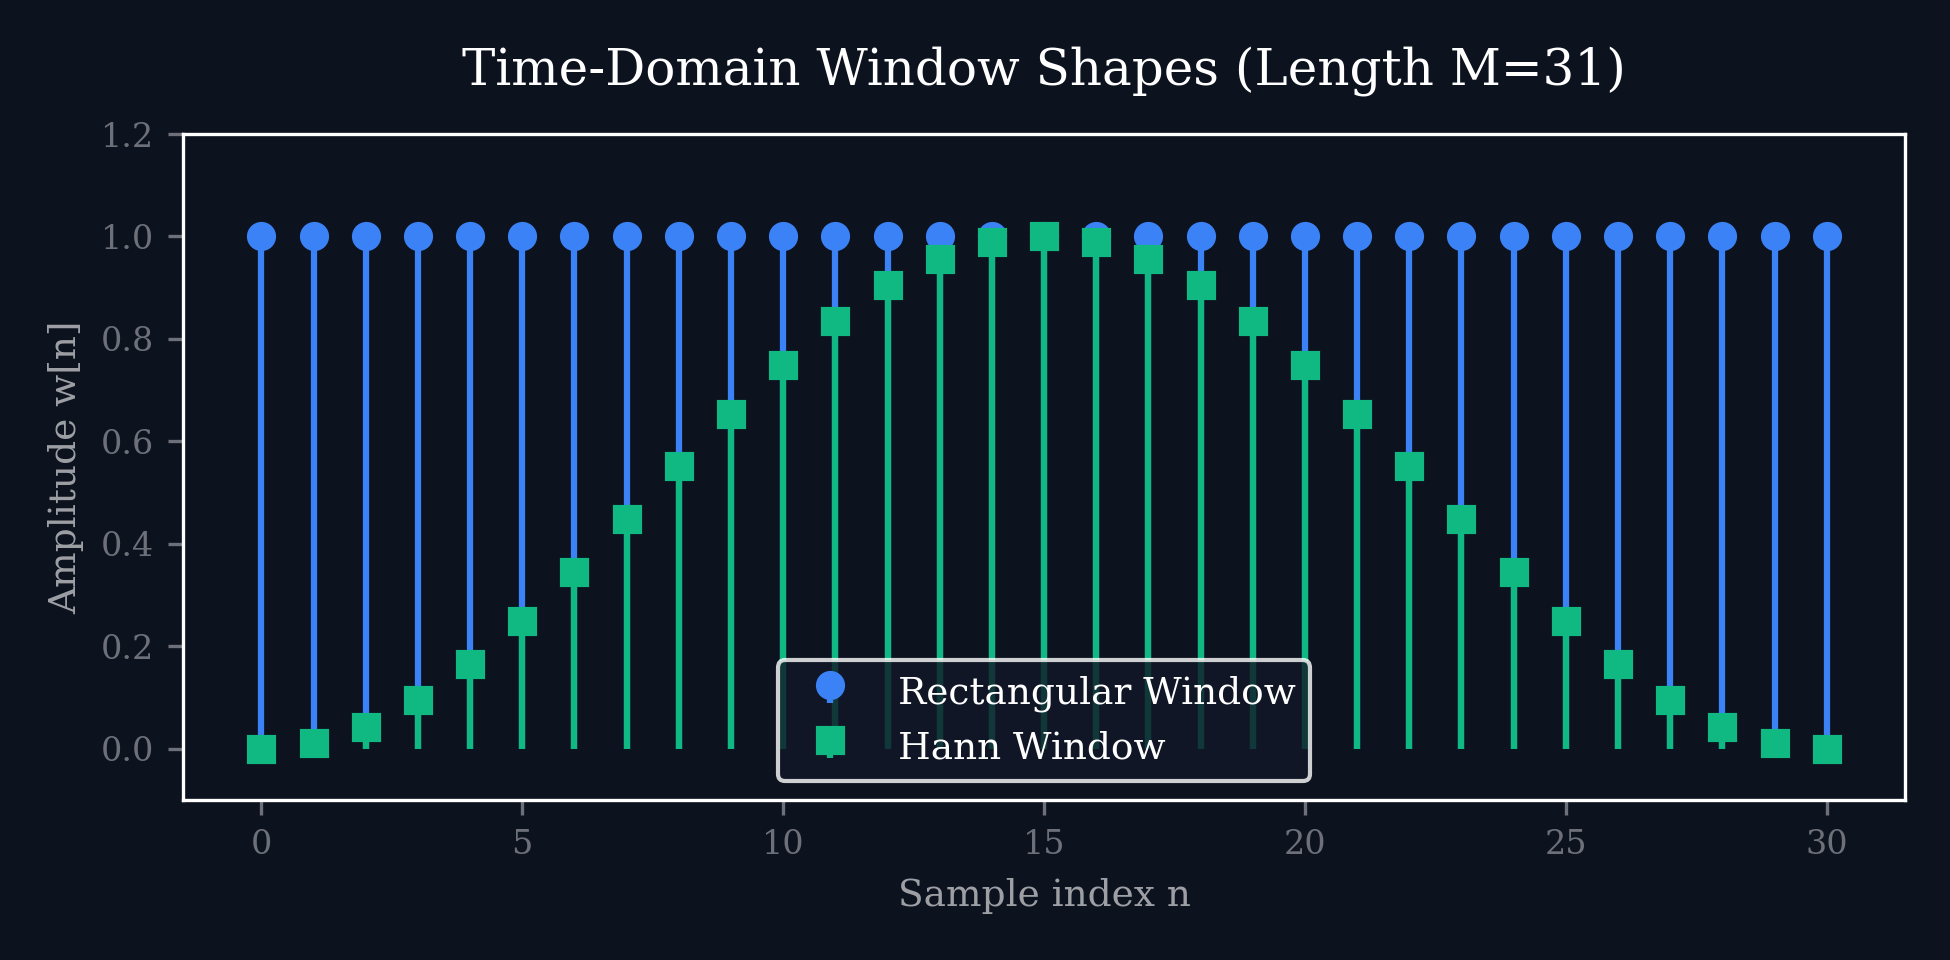
\includegraphics[width=0.75\textwidth]{images/window_shapes.png}
\caption{Time-domain shapes of windows used in interpolation filter design.}
\label{fig:window_shapes}
\end{figure}

A poor window choice (like rectangular) results in the Gibbs phenomenon, causing passband ripples and poor image rejection, as shown here:

\begin{figure}[H]
\centering
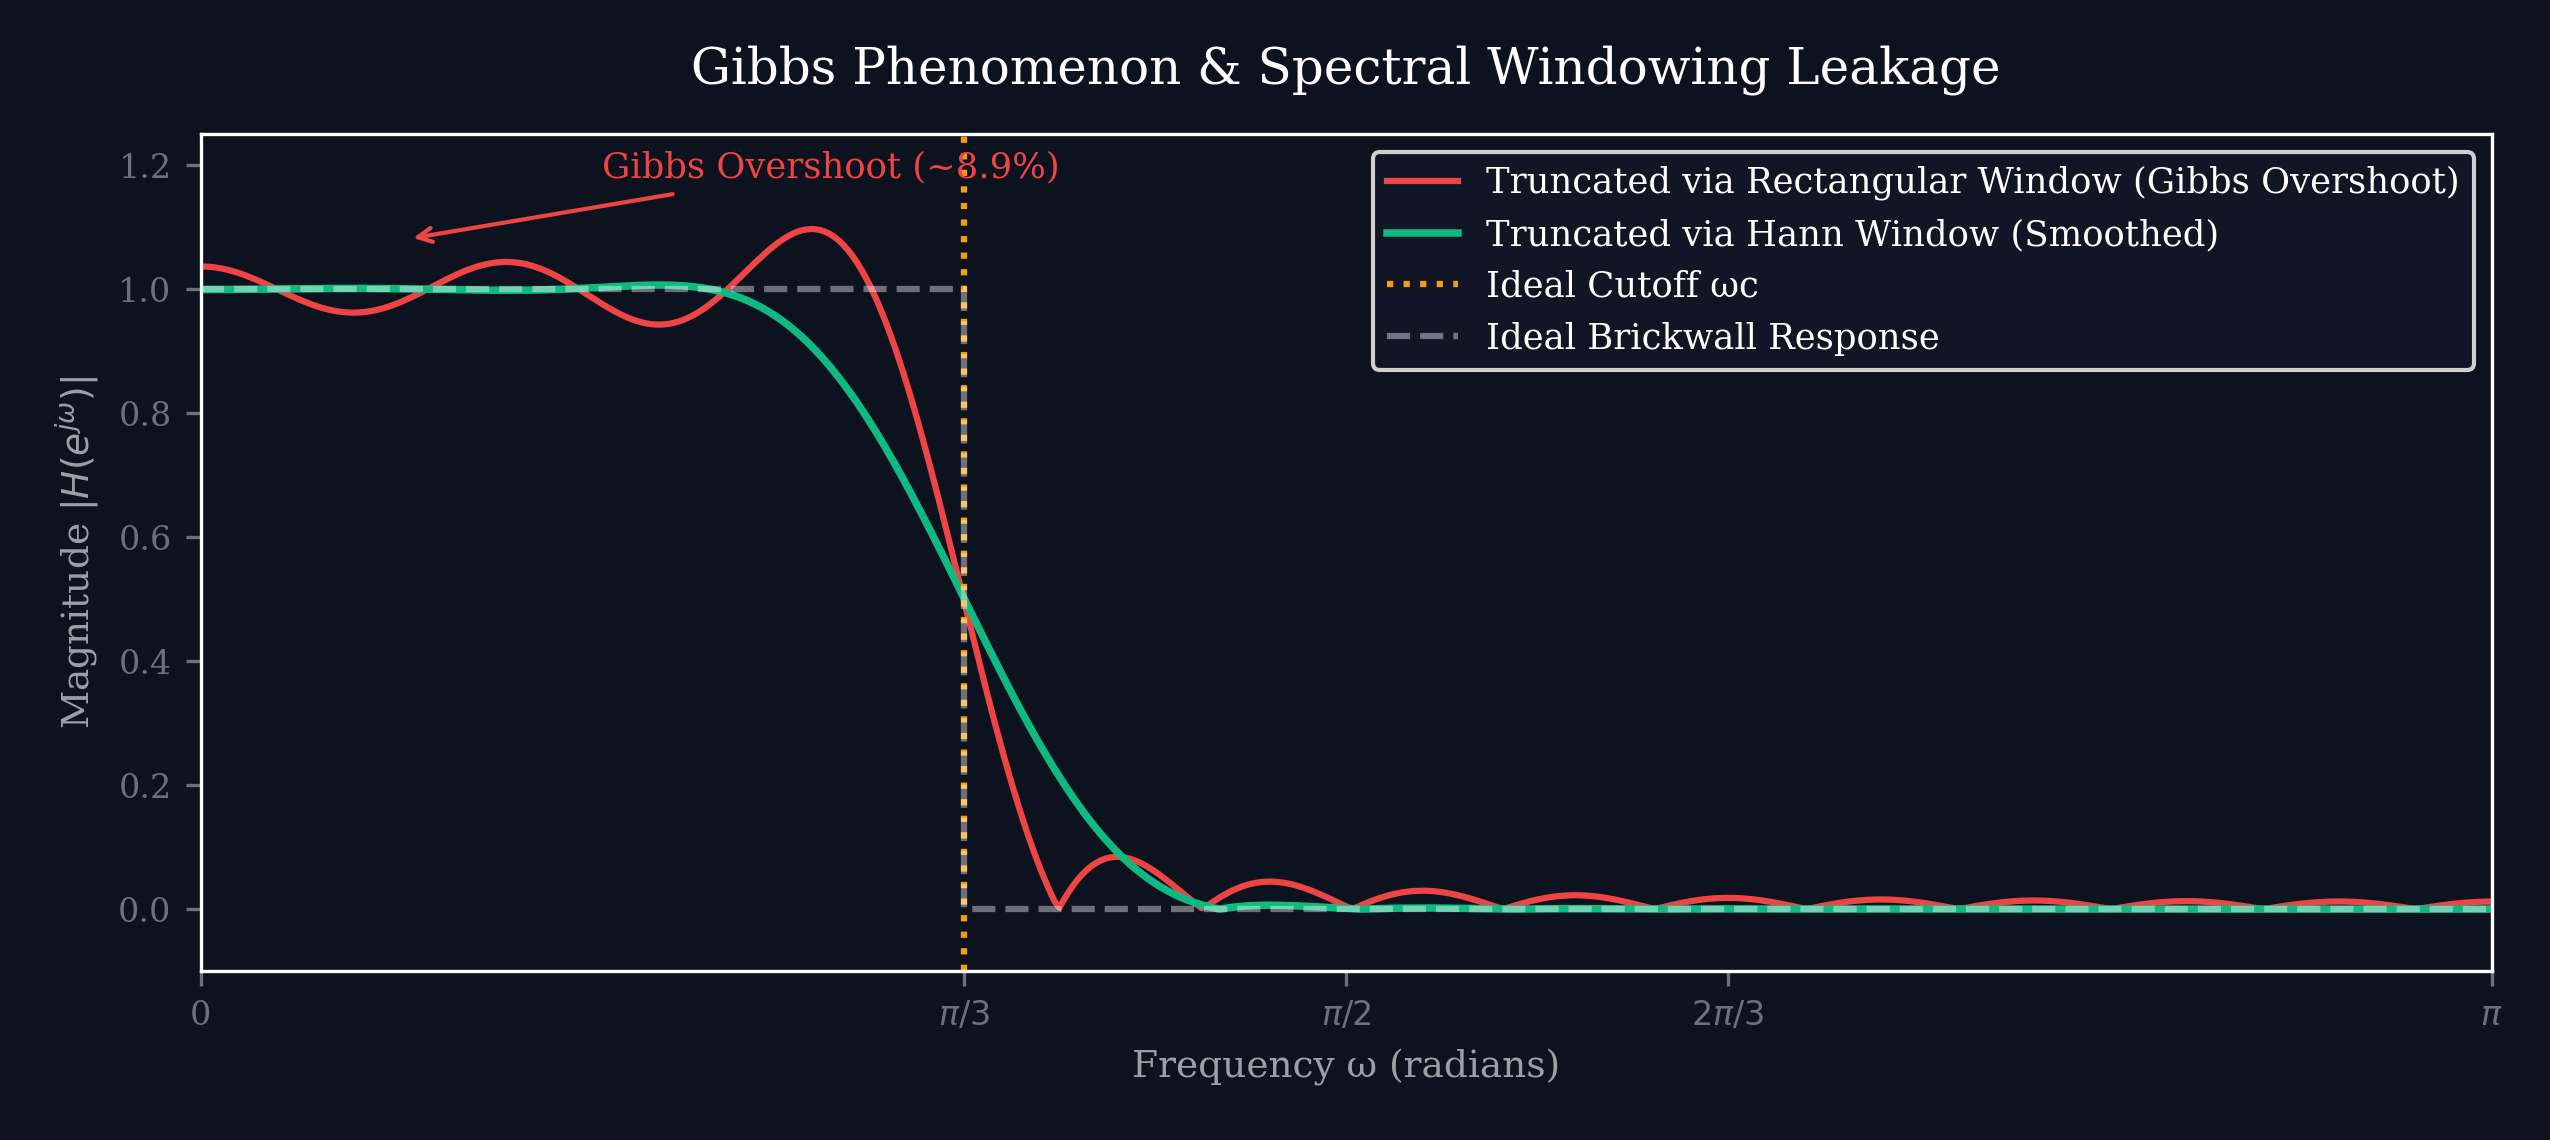
\includegraphics[width=0.85\textwidth]{images/gibbs_phenomenon.png}
\caption{Gibbs Phenomenon: Rectangular vs. Hann window responses.}
\label{fig:gibbs_comparison}
\end{figure}

\section{Oversampling ADC}
Oversampling means sampling at $k f_s$, where $f_s$ is the Nyquist rate and $k \gg 1$.

\subsection{Benefits of Oversampling}
\begin{enumerate}
    \item \textbf{Simplified Analog Anti-Aliasing Filter:} The transition band is massively widened.
    \item \textbf{Quantization Noise Reduction:} Noise power is spread evenly over $[0, kf_s/2]$.
    \item \textbf{Digital Filtering:} A digital lowpass filter removes noise outside the baseband $[0, f_s/2]$.
    \item \textbf{SQNR Improvement:} The Signal-to-Quantization-Noise Ratio (SQNR) improves by:
    \begin{equation}
        \Delta \text{SQNR} = 10 \log_{10}(k) \text{ dB}
    \end{equation}
\end{enumerate}

\section{Sigma-Delta ($\Sigma\Delta$) ADC}
Sigma-Delta ADCs combine massive oversampling with \textbf{noise shaping}.

\subsection{First-Order Noise Shaping}
By placing the quantizer inside a feedback loop with an integrator, the quantization noise is high-pass filtered. The noise transfer function (NTF) is $1 - z^{-1}$. First-order shaping provides a 9 dB SQNR improvement per octave.

\subsection{Second-Order Noise Shaping}
Using two integrators gives a second-order noise shaping:
\begin{equation}
    NTF(z) = (1 - z^{-1})^2
\end{equation}
This provides a 15 dB SQNR improvement per octave (2.5 bits), allowing a simple 1-bit quantizer to achieve 24-bit audio resolution after decimation!

\section{Sample Rate Conversion}
\subsection{Rational $L/M$ Factor Conversion}
If the ratio of the new rate to the old rate is a rational number $L/M$:
\begin{enumerate}
    \item \textbf{Interpolation:} Insert $L-1$ zeros between each sample.
    \item \textbf{Low-Pass Filter:} Apply a digital low-pass filter at the intermediate high rate to remove imaging.
    \item \textbf{Decimation:} Keep only every $M$-th sample.
\end{enumerate}
\subsection{Polyphase Filter Implementation}
The filter is decomposed into $L$ sub-filters (polyphase decomposition). This allows the filtering to happen at the lower sample rates.

\section{Key Formulas Table}
\begin{table}[H]
\centering
\begin{tabular}{ll}
\toprule
\textbf{Concept} & \textbf{Formula} \\
\midrule
Sampled Spectrum & $X_s(f) = f_s \sum_k X(f - kf_s)$ \\
Nyquist Criterion & $f_s \geq 2f_{max}$ \\
Ideal Reconstruction & $x(t) = \sum_n x[n]\text{sinc}(f_s t - n)$ \\
Aliased Frequency & $f_a = |f - kf_s|$ \\
ZOH Frequency Response & $H_{ZOH}(f) = T\text{sinc}(fT)e^{-j\pi fT}$ \\
Oversampling SQNR Gain & $10\log_{10}(k)$ dB \\
\bottomrule
\end{tabular}
\end{table}

\section{Checkpoints \& Quick Review Questions}
\begin{enumerate}
    \item \textbf{Q1:} An analog signal with frequency components up to 15 kHz is sampled at 20 kHz. Is the Nyquist criterion met? If a 12 kHz component exists in the signal, at what frequency will it appear in the sampled digital signal?
    \begin{itemize}
        \item \textit{Answer:} The Nyquist criterion requires $f_s \geq 2 f_{max}$. Here, $2f_{max} = 30$ kHz, but $f_s = 20$ kHz. Thus, the \textbf{Nyquist criterion is NOT met}. To find the aliased frequency of the 12 kHz tone, we use $f_a = |f - kf_s|$. For $k=1$:
        $f_a = |12 \text{ kHz} - 1(20 \text{ kHz})| = |-8 \text{ kHz}| = 8 \text{ kHz}$. The 12 kHz tone will appear as an \textbf{8 kHz alias}.
    \end{itemize}
    \item \textbf{Q2:} Explain physically why a Zero-Order Hold (ZOH) circuit introduces distortion (droop) in the reconstructed signal's passband, and how a digital interpolation filter can correct this.
    \begin{itemize}
        \item \textit{Answer:} Physically, holding a sample constant for duration $T$ creates a stair-step waveform. The flat part essentially acts as a low-pass averager in the time domain, which attenuates the higher frequencies of the original baseband signal. Mathematically, this is the $\text{sinc}(fT)$ frequency response. An interpolation filter can correct this by applying an ``inverse-sinc'' equalization in its passband to perfectly cancel out the ZOH attenuation before sharply cutting off to remove images.
    \end{itemize}
    \item \textbf{Q3:} Why does a Sigma-Delta ADC use a 1-bit quantizer instead of a multi-bit quantizer, given that 1-bit quantization introduces massive quantization noise?
    \begin{itemize}
        \item \textit{Answer:} A 1-bit quantizer is perfectly linear, eliminating the differential non-linearity (DNL) errors inherent in multi-bit resistor ladders. While 1-bit quantization adds huge noise, the feedback loop in the $\Sigma\Delta$ architecture performs \textbf{noise shaping}, pushing this noise to very high frequencies outside the signal band. Massive \textbf{oversampling} combined with a digital low-pass decimation filter completely removes this high-frequency noise, leaving an incredibly high Signal-to-Noise Ratio.
    \end{itemize}
\end{enumerate}

\end{document}
